%%%%%%%%%%%%%%%%%%%%%%%%%%%%%%%%%%%%%%%%%%%%%%%%%%%%%%%%%%%%%%%%%%%%%%%%%%%%%%%%
%%%%%%%%%%%%%%%%%%%%%%%%%%%%%%%%%%%%%%%%%%%%%%%%%%%%%%%%%%%%%%%%%%%%%%%%%%%%%%%%
%%%%%%%%%%%%%%%%%%%%%%%%%%%%%%%%%%%%%%%%%%%%%%%%%%%%%%%%%%%%%%%%%%%%%%%%%%%%%%%%
\section{Matrices de Wigner}
\label{app_matwig}
%%%%%%%%%%%%%%%%%%%%%%%%%%%%%%%%%%%%%%%%%%%%%%%%%%%%%%%%%%%%%%%%%%%%%%%%%%%%%%%%
%%%%%%%%%%%%%%%%%%%%%%%%%%%%%%%%%%%%%%%%%%%%%%%%%%%%%%%%%%%%%%%%%%%%%%%%%%%%%%%%
%%%%%%%%%%%%%%%%%%%%%%%%%%%%%%%%%%%%%%%%%%%%%%%%%%%%%%%%%%%%%%%%%%%%%%%%%%%%%%%%



%%%%%%%%%%%%%%%%%%%%%%%%%%%%%%%%%%%%%%%%%%%%%%%%%%%%%%%%%%%%%%%%%%%%%%%%%%%%%%%%
%\section{Introducción } %%%%%%%%%%%%%%%%%%%%%%%%%%%%%%%%%%%%%%%%%%%%%%%%%%%%%%%%

Se denominan funciones $D$ de Wigner, $D_{m,m'}^j(\alpha,\beta,\gamma)$, a los elementos de matriz del operador de rotaciones, $R(\alpha,\beta,\gamma)$, para un estado $|j\,m\rangle$ con valores bien definidos de momento angular $j^2$ y de su proyección $j_z$ \cite{kutschke1996angular}. De modo que
\begin{equation}
	\psi_{jm'}(\theta',\phi',\sigma') = R(\Omega) \psi_{jm} (\theta,\phi,\sigma) = \sum_{m' = -j}^j  \psi_{jm} (\theta,\phi,\sigma) D_{m,m'}^j(\Omega),
\end{equation}
siendo $\theta$ y $\phi \, (\theta'$ y $\phi')$ los ángulos polares iniciales (rotados) y $\sigma(\sigma')$ referida a las variables de espín. Además, se tiene la relación con las matrices $d$ de Wigner,
\begin{equation}
	D_{m,m'}^j (\alpha,\beta,\gamma) \equiv e^{-i\alpha m} d_{m,m'}^j (\beta) e^{-i\gamma m'}.
\end{equation}


Al considerar la desintegración del $\Bs$ en $\Jpsi$ y $\fai$, que a su vez decaen en $\muon \antimuon$ y  $\antikaon\kaon$ \footnote{Aunque los nombres de partículas sean específicos, este es un marco y procedimiento general para las desintegraciones a cuatro cuerpos que mediados por dos resonancias intermedias para desintegraciones escalares.}.
%
Los estados para las partículas se definen, por ejemplo, para el $\Jpsi$, como $\Jpsi:  |j_{\Jpsi} \,\lambda_{\Jpsi}\rangle$. Cuando $\Jpsi$ decae, se proyecta en un nuevo plano, $X_{\Jpsi}',Y_{\Jpsi}',Z_{\Jpsi}'$, cuya amplitud es proporcional a 
\begin{equation*}
\langle j_{\Jpsi},\, \lambda_{\muon} - \lambda_{\antimuon} | R(\alpha,\beta,\gamma) | j_{\Jpsi} , \lambda_{\Jpsi} \rangle \equiv D_{\lambda_{\Jpsi},\lambda_{\muon} - \lambda_{\antimuon}}^{j_{\Jpsi}}	(\alpha,\beta,\gamma)
\end{equation*}
es decir, precisamente la matriz de Wigner-$D$. Aquí $\alpha,\beta$ y $\gamma$
son los ángulos de Euler, que en la Mecánica Clásica  definen cualquier posible rotación en el espacio tridimensional. Hay otras convenciones posibles para estos ángulos, una de ellas --- y la usada por \lhcb --- es la convención de Jacobi--Wick \cite{kutschke1996angular}, que dicta
$R(\alpha,\beta,\gamma)  \rightarrow R(\alpha,\beta,-\alpha).  $


\begin{figure}[H]
\centering
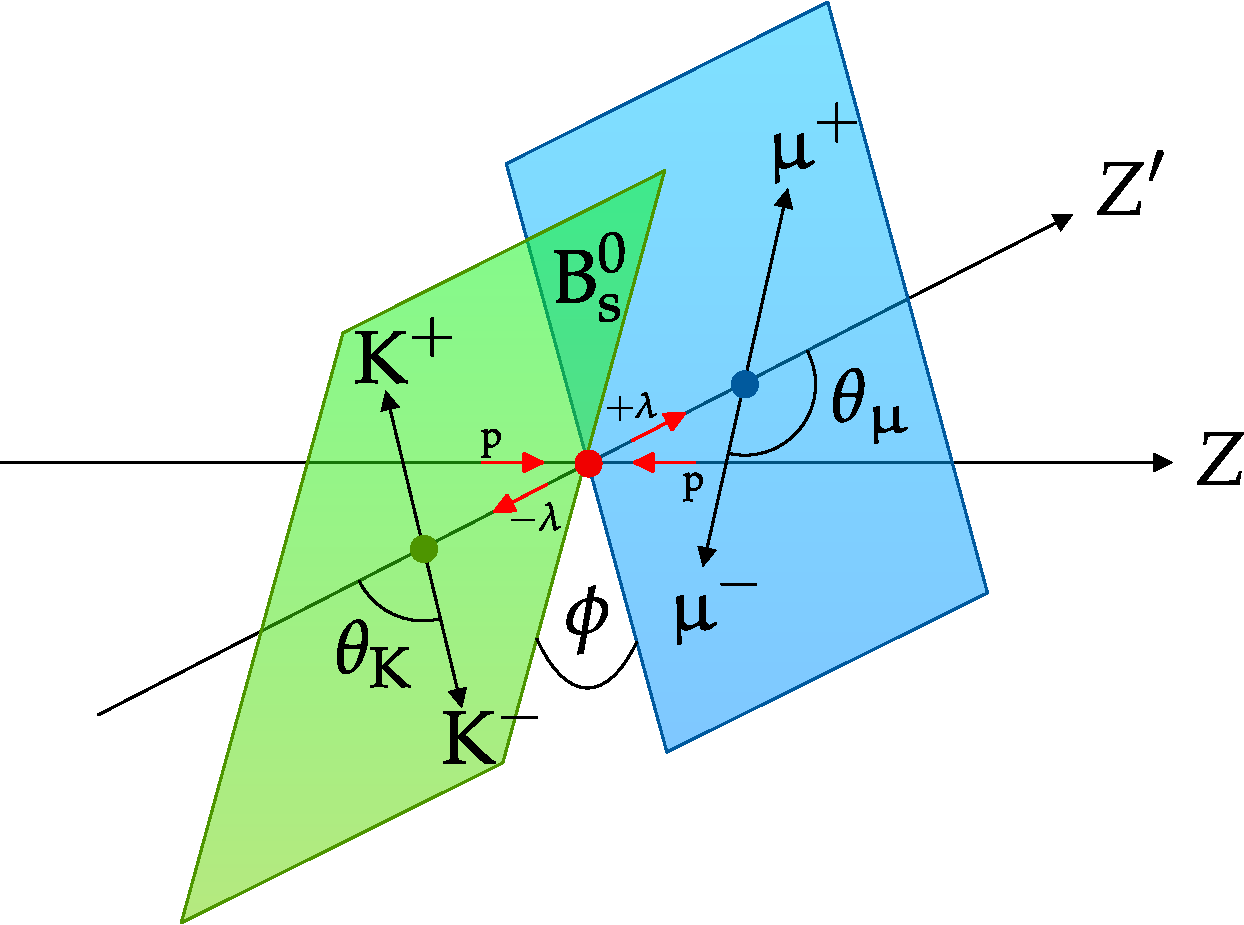
\includegraphics[width=0.48\textwidth]{WignerD1}
\hfill
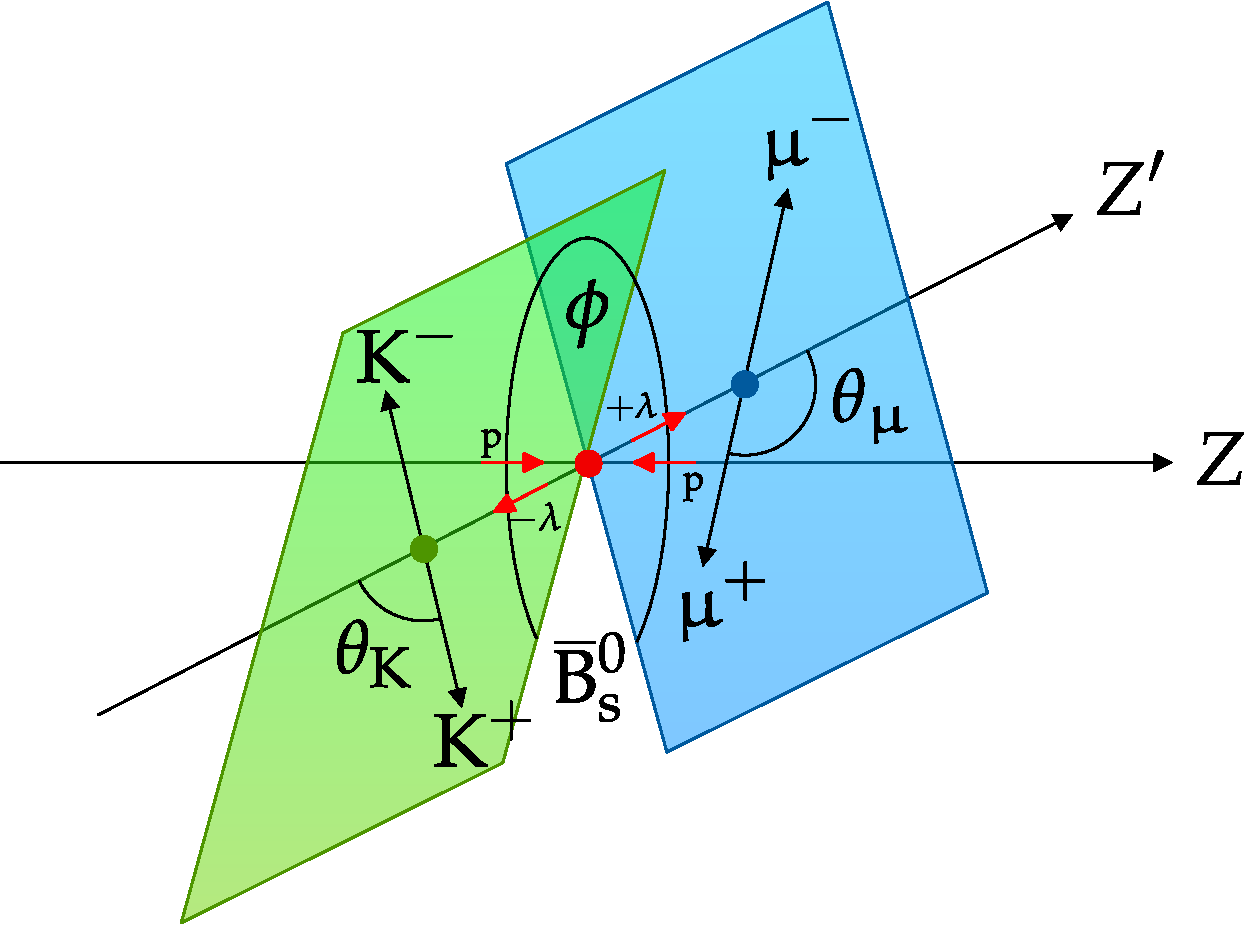
\includegraphics[width=0.48\textwidth]{WignerD2}
\caption{Definición de la helicidad y ángulos de helicidad para los desintegraciones $\Bs$ y $\Bbs$.}	
\end{figure}



%
Por tanto, la amplitud del proceso será proporcional al siguiente producto de funciones de Wigner
\[\mathcal{A} \sim D_{\lambda_{\Bs},\lambda_{\Jpsi}-\lambda_{\fai}}^{j_{\Bs}}\,D_{\lambda_{\Jpsi},\lambda_{\muon}-\lambda_{\antimuon}}^{j_{\Jpsi}}\, D_{\lambda_{\fai},\lambda_{\kaon}-\lambda_{\antikaon}}^{j_{\fai}}\]
Dado que el $\Bs$ carece de espín, $D_{0,\lambda_{\Jpsi}-\lambda_{\fai}}^0 = \delta_{0,\lambda_{\Jpsi}-\lambda_{\fai}}^0$, por lo que las helicidades del $\Jpsi$ y del $\fai$ deben ser contrarias respecto de la dirección del $\Bs$ (o equivalentemente, conservar el momento lineal). Así,
\[\mathcal{A} \sim D_{\lambda_{\Jpsi},\lambda_{\muon}-\lambda_{\antimuon}}^{j_{\Jpsi}}\, D_{\lambda_{\fai},\lambda_{\kaon}-\lambda_{\antikaon}}^{j_{\fai}},\]
o denominando $\lambda \equiv \lambda_{\Jpsi} = - \lambda_{\fai} $, $\alpha = \lambda_{\muon}-\lambda_{\antimuon}$, $j \equiv j_{\fai}$ y como los kaones son escalares \cite{zhang2013time},
\begin{equation}
\begin{split}
\mathcal{A} &  \sim D_{\lambda,\alpha}^{1}(0, \theta_{\upmu}, 0)\, D_{-\lambda,0}^{j} (\phi, \theta_{\text{K}} , -\phi ) = \\
&= d_{\lambda,\alpha}^{1} (\theta_{\upmu})\, e^{-i (-\lambda) (\phi)} d_{-\lambda,0}^{j}(\theta_{\text{K}}) e^{-i (0) (-\phi)} = \\ 
&= e^{i\lambda \phi} \,d_{\lambda,\alpha}^{1} (\theta_{\upmu})\,  d_{-\lambda,0}^{j}(\theta_{\text{K}}) .
\end{split}	
\end{equation}
encontrando así la notación estándar de los términos angulares de la amplitud.



%%%%%%%%%%%%%%%%%%%%%%%%%%%%%%%%%%%%%%%%%%%%%%%%%%%%%%%%%%%%%%%%%%%%%%%%%%%%%%%%
%%%%%%%%%%%%%%%%%%%%%%%%%%%%%%%%%%%%%%%%%%%%%%%%%%%%%%%%%%%%%%%%%%%%%%%%%%%%%%%%
%%%%%%%%%%%%%%%%%%%%%%%%%%%%%%%%%%%%%%%%%%%%%%%%%%%%%%%%%%%%%%%%%%%%%%%%%%%%%%%%